\section{三维测距技术}
近年来,三维测距技术得到了越来越广泛的应用。
传统的的三维测距技术通常应用在w专业的三维扫描设备中,
但今年来越来越多的公司都推出了搭载三维测距技术的产品与项目,
如Microsoft的Kinect\cite{microsoft_kinect}、
Google的Tango\cite{google_tango} Project,
Apple的iPhone X\cite{apple_iphoneX}、Intel的RealSense\cite{intel_realsense}等。
三位测距技术可分为主动测距和被动测距。其中主动测距需要由辐射源将额外能量辐射到物体表面,
根据物体表面反射的能量进行测距。被动测距则不需要设置辐射源,只利用二维图像来重建场景的三维信息。

\begin{figure}[h]
    \centering
    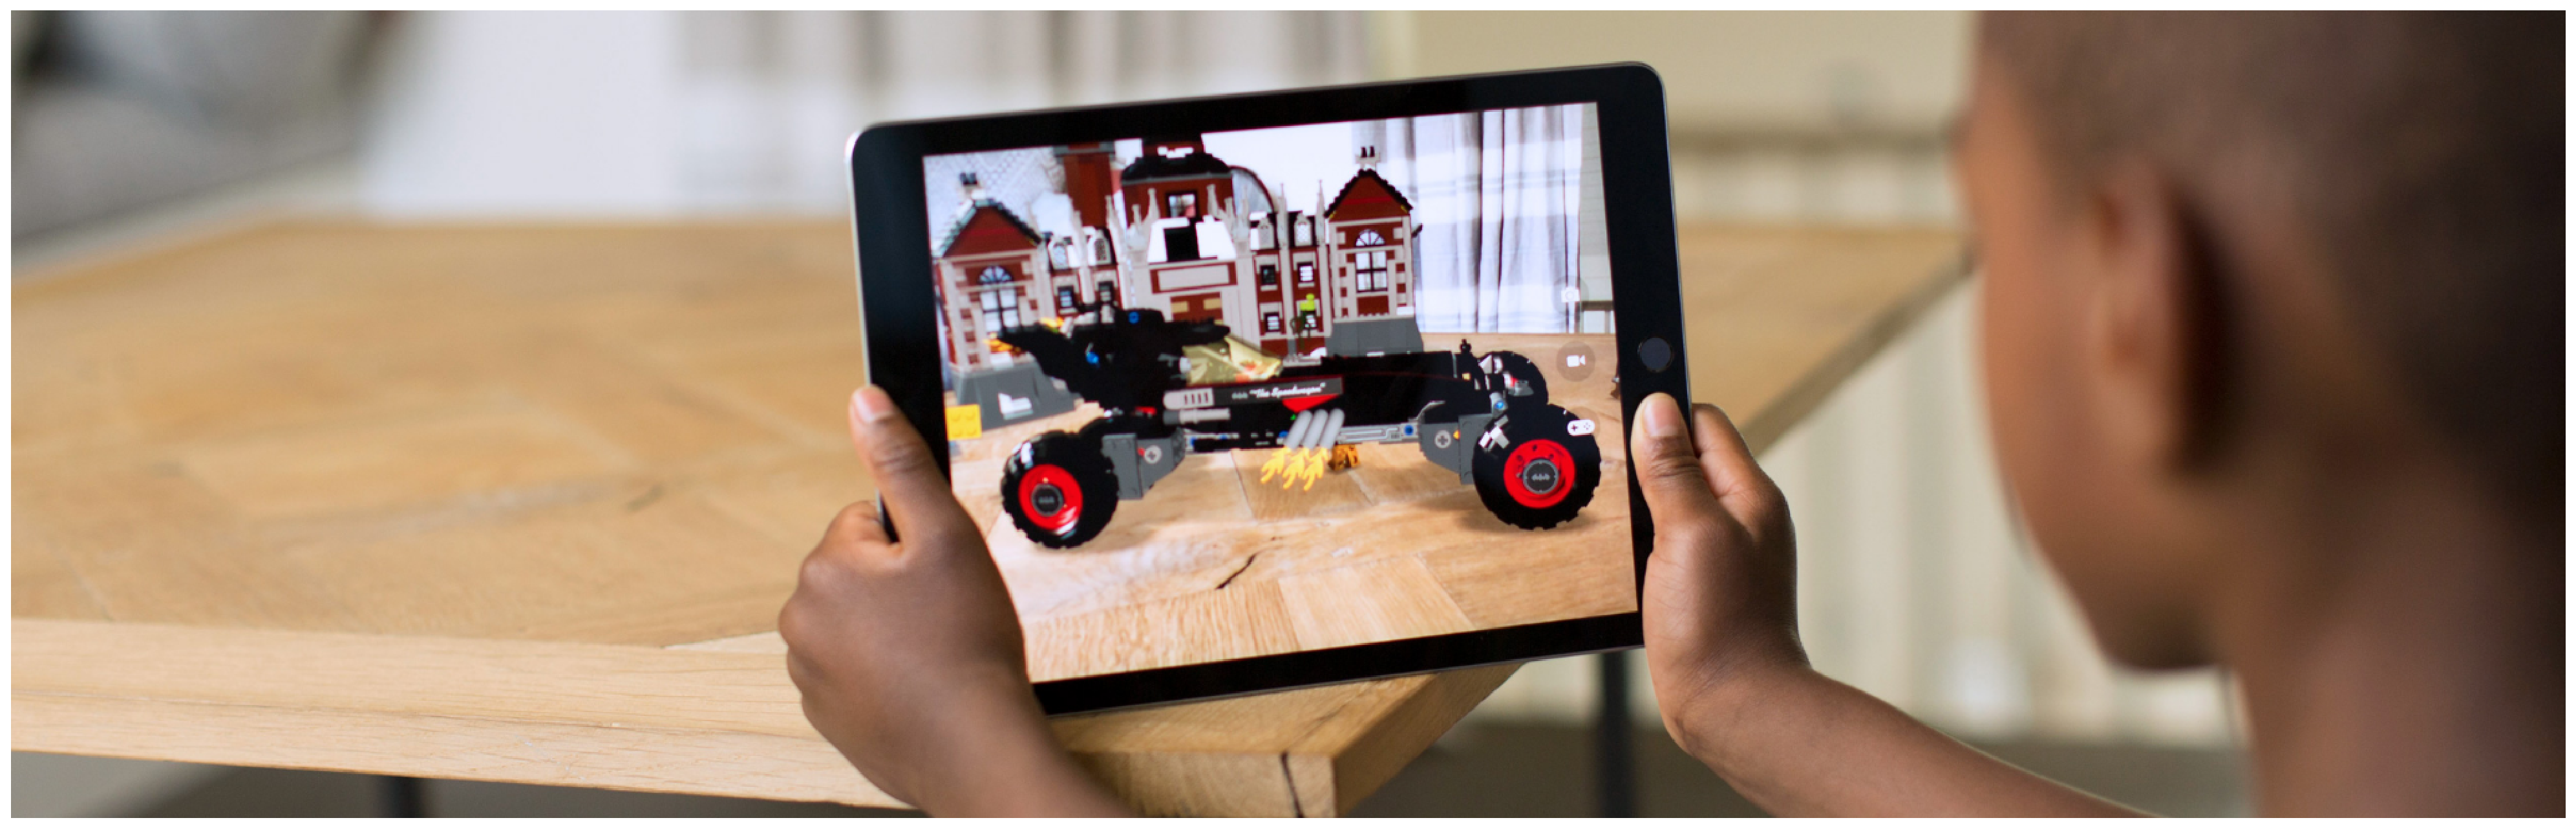
\includegraphics[width=0.95\textwidth]{./Pictures/ARKit.eps}
    \caption{Apple ARKit}
    \label{arkit}
\end{figure}
现在主流的被动测量技术主要基于立体视觉(Stereoscopic),通常通过区块匹配(block matching)或对极几何(epipolar geometry)算法实现。
此外随着运动传感器技术的成熟与普及,
越来越多的视觉SLAM(Simultaneous Localization and Mapping,即时定位与地图构建)系统会借助
IMU(Inertial Measurement Unit,惯性测量单元),如Apple的ARKit\cite{apple_arkit},如图\ref{arkit}。

主流主动测距技术有飞行时间(ToF,Time-of-Flight)、
三角测距(Triangulation)和结构光(Structured light)。本文使用的是基于主动测距技术的深度相机。
\subsection{飞行时间测距}
飞行时间测距,又称为激光雷达(LiDAR)测距法。
激光发射器会将激光脉冲投射到物体表面,相应的传感器会接收物体表面反射的激光信号,
控制器就会根据信号传播所消耗的时间计算出相应监测点和传感器的距离。但由于光速(\(299792458 m/s\))非常快,
直接测量飞行时间是不现实的。例如测量1m的距离,飞行时间为\(1/299792458 \times 2\)s,
相机的采集平率需达到\(1.5 \times 10^8\)Hz,这个是硬件很难达到的。
因此,基于飞行时间的设备会发射固定频率调制的正弦光波,摄像头同步摄像头同步拍摄多帧反射图像,
根据每个像素亮度的变化规律计算反射光的相位差。
相位差再乘以光速就得到了像素的距离,如图\ref{tof}。

\begin{figure}[h]
    \centering
    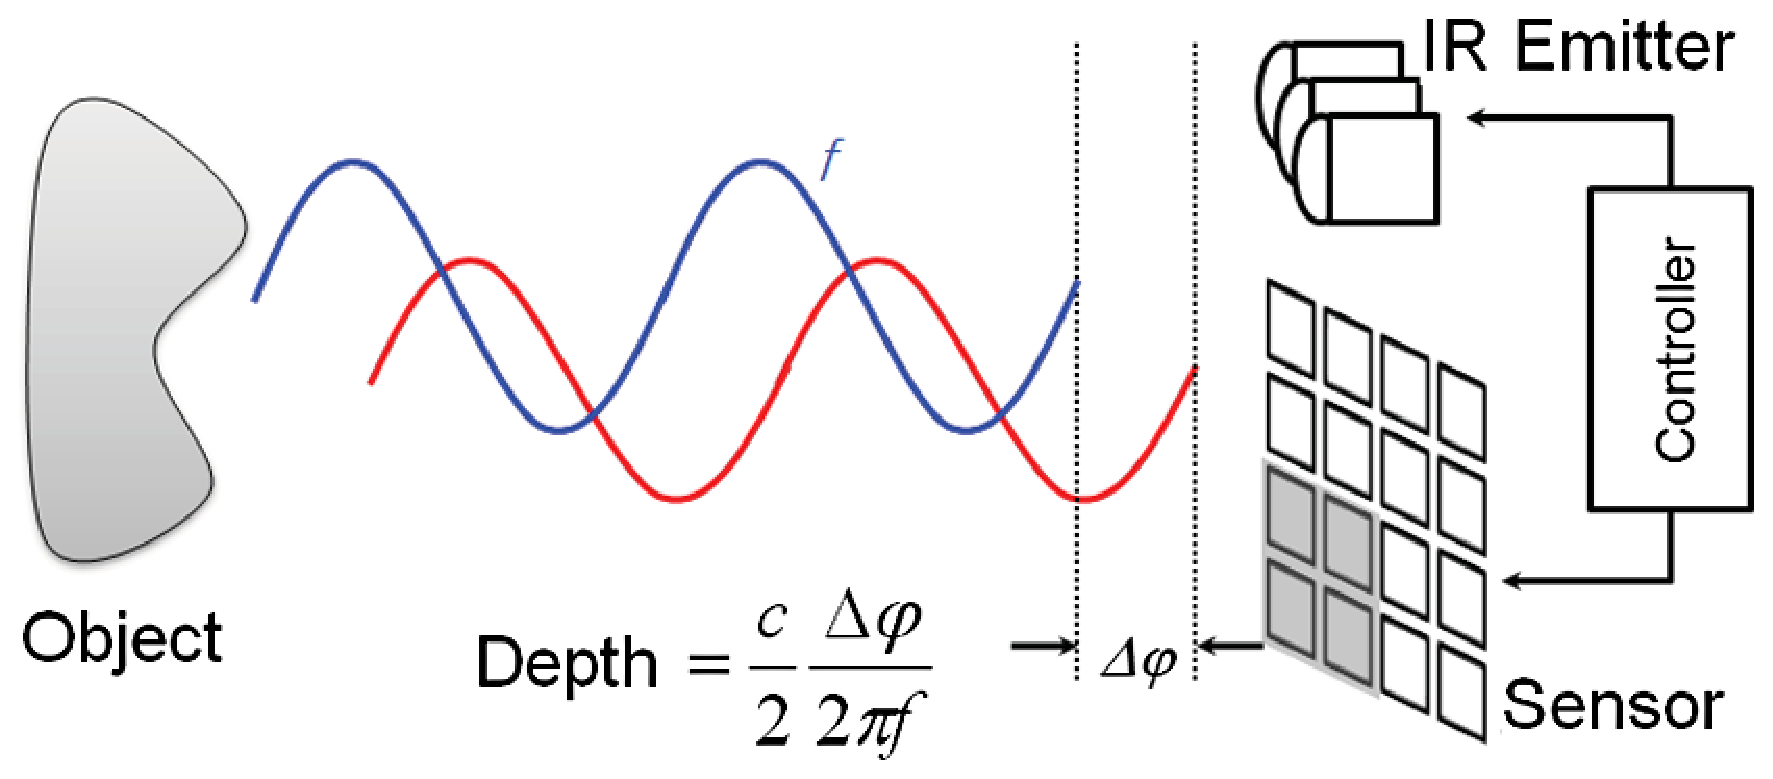
\includegraphics[width = 0.95\textwidth]{./Pictures/TOF.eps}
    \caption{ToF测距原理}
    \label{tof}
\end{figure}
\subsection{三角测距}

三角测距法又称主动三角法,
是基于光学三角原理,根据光源、物体和检测器三者之间的几何成像关系来确定空间物体各点的三维坐标,如图\ref{triangulation}。
在实际测量过程中,它常用激光作为光源,用CCD相机作为检测器。
这种方式主要用于工业勘探、工件表面粗糙度检测、轮胎检测、飞机检测等工业、航空、军事领域,
在消费电子类产品还不曾涉及。

\begin{figure}[h]
    \centering
    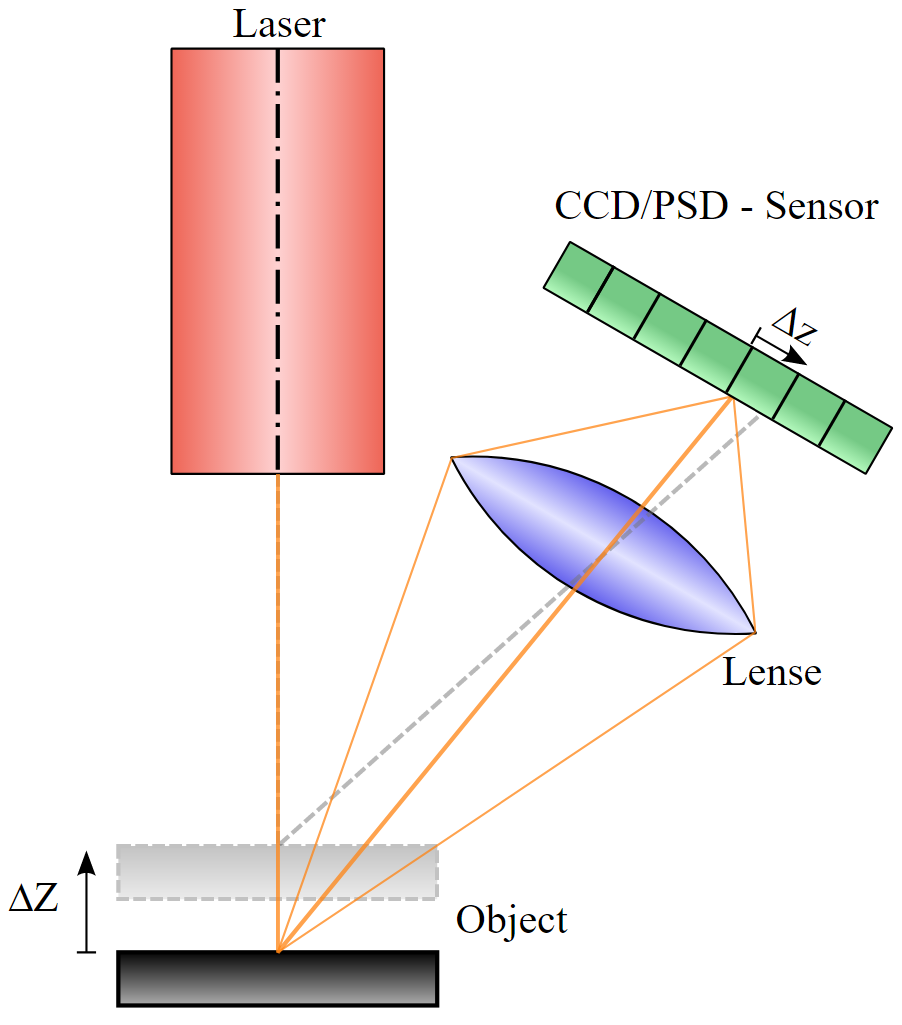
\includegraphics[width = 0.5\textwidth]{./Pictures/Triangulation}
    \caption{三角测距原理}
    \label{triangulation}
\end{figure}




